\chapter{Motion Planning}

% Alternative outlay: Overview -> Representation (discrete, cont, determ, prob,
% state-space implici/explicit)

\section{Overview/Preliminaries}
Motion planning is the task of manipulating a robot's configurations so that,
given an initial and goal state or posture, the planner (black box), is able to
create a sequence of actions that gives a feasible or optimal path through the
overarching planning environment, usually referred to as the world space. Thus a
motion planner can be seen as a machine which given an input: a world, and
initial and goal states, produces a sequence of actions to move the robot from
its initial to the desired goal configuration. This plan is then passed on to
the trajectory generator in the system. Generally, planners can be separated
into complete and non-complete planners, meaning that given enough time, all
motion planning problems are solvable, only the solution is NP-Hard. Thus
feasible solutions will have to make a compromise, and a lot of planners in use
today are what is called probabilistically complete, meaning that they converge
to a perfect solution given infinite time. As such time-frames are of no use to us, we
generally have to settle for an approximation bound. There is a difference
between online and off-line motion planning, whereas the offline algorithm plans
in a static environment, the online algorithm is run continuously. However an
online algorithm can be simulated by running an offline algorithm repeatedly for
short intervals of time. However, this comes with the drawback, that no
guarantee can be made for completing a certain task.

\subsection{Building Blocks}

\subsection{The Robot and World Model}

The modeled world \(\modelworld\), and everything in it can be modeled
geometrically using any number of methods - most usually polygons or some other
convex geometric structure. Thus the robot can also be modeled as a collection
of geometric structures \(\modelrobot\). Thus in order to move the robot in the
world space, rigid body transformations are applied. Given the robot as a subset
of the world space, the image of a robot transformation is then given as:
% \[
%   h(\modelrobot) = \set{h(a) \in \modelworld \mid a \in \modelrobot} \\
%   h \colon \modelrobot \rightarrow \modelworld \\
%   \modelrobot \and h(\modelrobot) \subset \modelworld \\
% \]

The world as we model it contains two kinds of objects

\begin{itemize}
\item \textbf{Robot:} Body that is modeled geometrically and is controllable via
  a motion plan.
\item \textbf{Obstacles:} Portions of the world that are occupied by something
  other than the robot.
\end{itemize}

\subsection{Rigid Transformations}

% \subsection{State Space}
% \label{subsec:State}
% Planning problems involve a state space. A state space is a set of all the
% possible configurations a model can be in at any given time. The state space
% can be either discrete or continuous, and can be represented either implicitly
% or explicitly.

\subsubsection{Configuration Space}
The configuration space is a general abstraction used as a model for a wide
variety of motion planning problems. It is a manifold that arise from the
transformations applied to the robot. If the robot has n-degrees of freedom, the
set of transformations is usually a manifold of dimension n. This manifold is
called the configuration space of the robot, and is shortened
\(\modelconfigurationspace{}\). Thus in order to solve a motion planning
problem, a search must be performed in the configuration space. Thus the motion
planning problem is now made into a question of finding the best path to
traverse the given manifold\cite{Lav06}. (characterize and describe the
configuration space structure.) In our case the configuration space can be
modeled as a topological space of the type \(SE(3)\), meaning special-Euclidean
three.

Using generalized coordinates, the configuration of a robot can be modeled as a
vector with n variables for the position in the configuration space, in
literature this space is usually denoted by \(\modelconfigurationspace{}\). As
is most common, the robot is modeled as a rigid body, in which two bodies cannot
overlap, thus points in the configuration space is separated into two sets. One
set for which the robot configuration overlaps with another object in the
configuration space, and is called \(\modelconfigurationspaceobst{}\), and given
that the world space is represented as \(\modelconfigurationspace{}\), the
collision free space is the given as, \(\modelconfigurationspacefree =
\modelconfigurationspace \setminus \modelconfigurationspaceobst\). The obstacle
space can be represented in a number of ways, but we will stick to polygonal
models of the obstacle space.

\subsection{Action Space}
The action space is the set of actions that can be applied at any given state
the robot is located in. Thus one can model the action space as a function of
the robot's state.\ e.g.
\[
  \modelactionspace(x) = \set{u \in \modelactionspace \mid \modelactionspace(x)
    \neq \emptyset }
\]

\subsection{Initial and Goal States}
It is normal to define an initial state and a goal state as a starting and an
ending point of a planning problem. Where both the initial, and goal states can
be sets of states, meaning that it is not necessary to arrive specifically at
the target point. A starting point consisting of multiple configuration states
usually infers some kind of uncertainty in the robot model. The end goal can be
reached in one of two ways, wherein the two types characterize two different
forms of planning.
\begin{enumerate}
\item\textbf{Feasible:} Feasible planning has no concerns with optimality, and
  only concerns itself with finding a plan that arrives at the goal state.
\item\textbf{Optimal:} Optimal planning optimizes a feasible plan in some
  specified manner, with respect to some specified cost function.
\end{enumerate}

\subsection{A Plan}
If we are dealing with a fully deterministic model, a plan can simply be the set
of actions applied at each state in order to reach a goal state specified for
the problem at hand. However, if some measure of uncertainty is added to the
model, then literature describes this as planning in the \textit{information
  space}, and future states cannot be predicted exactly, thus some kind of
feedback model is used in order to plan in an uncertain environment. If we are
merely looking at solving the problem, a feasible plan is good enough, which
means a solution has to be found, but multiple solutions do not have to be found
and compared. However, if time, energy or some other parameters are to be
optimized, then a cost function has to be added into the planning model, in
order to evaluate which plan scores best when measured up against the others.

\subsection{Model}

\subsubsection{Discrete}
let \(\mathcal{X}\) be the discrete state space, and \(\mathcal{U}(x)\) be the
set of actions available at each point \(x \in \mathcal{X}\). State transition:\
\[
  x_{k+1} = f(x_k, u_k)
\]

\subsubsection{Continuous}

\subsubsection{Path and Trajectory}

The motion plan takes the form of a path, or a trajectory. This is represented
as a function \(\phi(\alpha) \colon [0,1] \rightarrow \mathcal{X}\), where
\(\mathcal{X}\) is the configuration space of the vehicle. If the
control-execution time is considered, then the explicit model of vehicle
kinematics and/or dynamics, as well as the dynamics of the possible obstacles.
Then the trajectory is represented as a time-parameterized function of the kind
\(\pi(t) \colon [0,T] \rightarrow \mathcal{X}\), where \(T\) is the planning
horizon. Unlike the path, the trajectory describes how the configuration of the
vehicle evolves over time.

Initial and Goal States. A path is a function f \ldots

\subsection{Time}

Discrete vs Continuous

\subsection{Actions}

A plan is a sequence of actions that manipulate the state of the robot. A
planning problem involves a sequence of decisions made over time. car-like model
can look something like:

\section{Algorithms}
In general there are algorithms for which every motion planning problem can be
solved explicitly, only their running time is on the order of \(O(n!)\) (TODO - cite!), and
thus not feasible in practical applications. In the practical case it is
therefore normal to employ methods of approximation.

\subsection{Grid-based Search}

\subsection{Interval-based Search}

\subsection{Geometric Algorithms}

\subsection{Artificial Potential Fields}

\subsection{Sampling-based}

\section{Piano Movers Problem}

\section{Discrete vs Continuous}

\section{Sampling}

\section{State Space}

\section{Complexity}

\section{Criterion}

\subsection{Feasibility}
\subsection{Optimality}

\section{Completeness}

\section{Probabilistic Completeness}

\section{Planning Under Uncertainty (Decision Theoretic Planning)}

All real life motion planning problems are faced with some level of uncertainty,
as errors can arise from a multiple of sources, whereas the most prevalent ones
are uncertainty in:
\begin{enumerate}
\item motion
\item sensing
\item the environment
\end{enumerate}
Thus the exact system state is never exactly known. Therefore planning under
uncertainty is done in a belief space. Which is a description of the state space
using probability distributions. (Partial observability?) Planning is done in
the information space, as opposed to the state-space. Uncertainties in
prediction and the current state exist. Forward and backward projections.

(probability constraint violation)

\subsection{A Game Against Nature}

Theta is nature's actions. U is the robot's action.

\subsection{A Model of Uncertainty}

If the discrete state space model is expanded to include \(\ Theta\) as the
space of nature actions, and \(\ theta_k\) is the action selected by nature at
step k, then a transition is modeled as
\[
  x_{k+1} = f(x_k,u_k,\theta_k)
\]
As the actions of nature are not available beforehand, that is -- \(\theta_ k\)
is not given, thus we have
\[
  X_{k+1} = \set{ x_{k+1} \ in X \mid \exists\theta_k \in \Theta(x_k,u_k)
    \text{such that } x_{k+1} = f(x_k,u_k,\theta_k)}
\]\cite{Lav06}.

\subsection{Discrete Planning with Nature}
a model of discrete planning with nature:~\cite[pg,496]{Lav06}

A Markov decision process is defined in~\cite[pg.498]{Lav06} as:
\begin{enumerate}
\item A non empty \textit{state space} \(X\) which is a finite or countably
  finite set of \textit{states}.
\item For each state, \(x \in X\), a finite non-empty \textit{action space}
  \(U(x)\). It is assumed that \(U\) contains a special \textit{termination
    action}, which has the same effect as (cite the deterministic discrete
  planning model).
\item A finite non-empty \textit{nature action space} \(\Theta(x,u)\) for each
  \(x \in X\) and \(u \in U\).
\item A state transition function \(f\) that produces a state,
  \(f(x,u,\theta)\), for every \(x \in X\), \(u \in U\), and \(\theta \in
  \Theta\).
\item A set of \textit{stages}, each denoted by k, that begins at k=1 and
  continues indefinitely. Alternatively, there may be a fixed maximum stage \(k
  = K+1=F\).
\item An \textit{initial state} \(x \in X\). For some problems, this may not be
  specified, in which case a solution plan must be found from all initial
  states.

\item A \textit{goal set} \(X_G \subset X\).
\item A stage-additive cost functional L. Let \(\sim{\theta}_K\) denote the
  history of nature actions up to stage K. The cost functional may be applied to
  any combination of state, action, and nature histories to yield
  \[
    L(\sim{x}_F, \sim{u}_K, \sim{\theta}_K) = \sum_{k=1}^{K} l(x_k,u_k,\theta_k)
    + l_F(x_F)
  \]
  in which \(F = K + 1\). The termination action \(u_T\) is applied at some
  stage k, then for all \(i \geq k\), \(u_i = u_T\), \(x_i = x_k\), and
  \(l(x_i,u_T, \theta_i) = 0\).
\end{enumerate}~\cite[pg 498]{Lav06}

using this formulation either a feasible or optimal planning problem can be
formulated.

\subsection{Forward and Back-Projections (under uncertainty)}

\subsection{Separating a plan from its execution}

\subsection{Feedback}

\subsection{Information Space}
A stochastic environment. The information space is a general structure for
working with plans under conditions of uncertainty. Thus planning can be done
mostly as it is done in a state space, albeit in a higher dimension. Thus the
state transition function can be written as
\[
  \phi_{k+1} = f_{\mathcal{I}}\left( \phi_k, \mu_k, y_{k+1} \right)
\]

\subsection{Nondeterministic and Probabilistic Information Spaces}

\subsection{A Plan under Uncertainty}
Since it Expected-case analysis. Worst-case analysis.

Uncertainty comes from three sources in our model:
\begin{enumerate}
\item The Model (motion).
\item The observation (sensor).
\item The environment (map). Grid-based problems: Navigation: A goal position is
  to be reached, even though the map is unknown. The robot is allowed to solve
  the problem without fully exploring the environment. Only a part of the
  environment is needed to solve the problem. Searching: A goal state can only
  be identified when it is reached by a short-range sensor. The environment is
  systematically searched, but the search may terminate early if the goal is
  found.

  Problem-definition: Part of the problem is map-building, as the map is not
  provided exactly, and sensory map-information has to be used in order to
  successfully solve a given planning problem.
\end{enumerate}

\subsection{Visibility Polygon}
Let \(V(x)\) be the visibility polygon -- that is the set of all points that are
visible from \(x\).

I-states enables us to solve problems without having a complete representation
of the environment! (LAV06) chp12.2



\subsubsection{Decision Makers}

\subsection{Rewards?}

\section{Data Collection and Sensors}



\section{Optimality}

\section{Misc}

\begin{table}
  \begin{tabular}{c c c p{4cm}}
    \hline
    \hline
    Algorithm Group & Technique & Variations & Description \\
    \hline
                    &  Dijkstra's Algorithm & &Algorithm for finding the shortest weighted path in a graph.\\
                    &  \\
    Graph Search               & & D* & Capable of planning paths in unknown, partially known, and changing environments in an efficient, optimal, and complete manner..\\
                    & A* Family & Focused-D* & Informed-incremental heuristic search.\\
                    & & D*-Lite & Simpler to implement that Focused D*, slightly slower performance.\\
    \hline
                    & RRT-implementations \\
                    & & RRT\\
                    & & RRT*\\
    Sampling based Planners& & RRT*-Smart\\
                    & & RRT-SLAM\\
                    & & CC-RRT\\
                    & PRM \\
                    & & BRM & A road-map implementation that plans in belief space in order to handle uncertainties in the planning model.\\
    \hline
    Numerical Optimization &  Function Optimization \\
    \hline
  \end{tabular} 
\end{table}

\section{Planning with Funnels}

A \textit{Funnel} is a parametrization of the reachable set of a dynamical
system. This means that a \textit{Funnel} holds all the states the dynamical
system can be in during a planning task. Mathematically we can define the
reachable set of the system as
\[
  \bar{x}(0) \in \mathcal{X}_0 \Rightarrow \bar{x}(t) \in F(t), \forall t \in \sqb{0,T}
\]
where \(\mathcal{X}_0\) is the set of initial conditions, \(\sqb{0,T}\) the time
interval, and \(F(t)\) is the set of states that the system can be in at time
\(t\). Although this thesis concerns itself with approximating the reachable set
through \textit{Lyapunov} functions, a useful analogy is imagining the funnel
created through \textit{Monte-Carlo} simulation, where the \textit{Funnel} would
be the set of all the paths traversed by the dynamical system at hand. For a
simple car model, this could look similar to:

\begin{figure}
  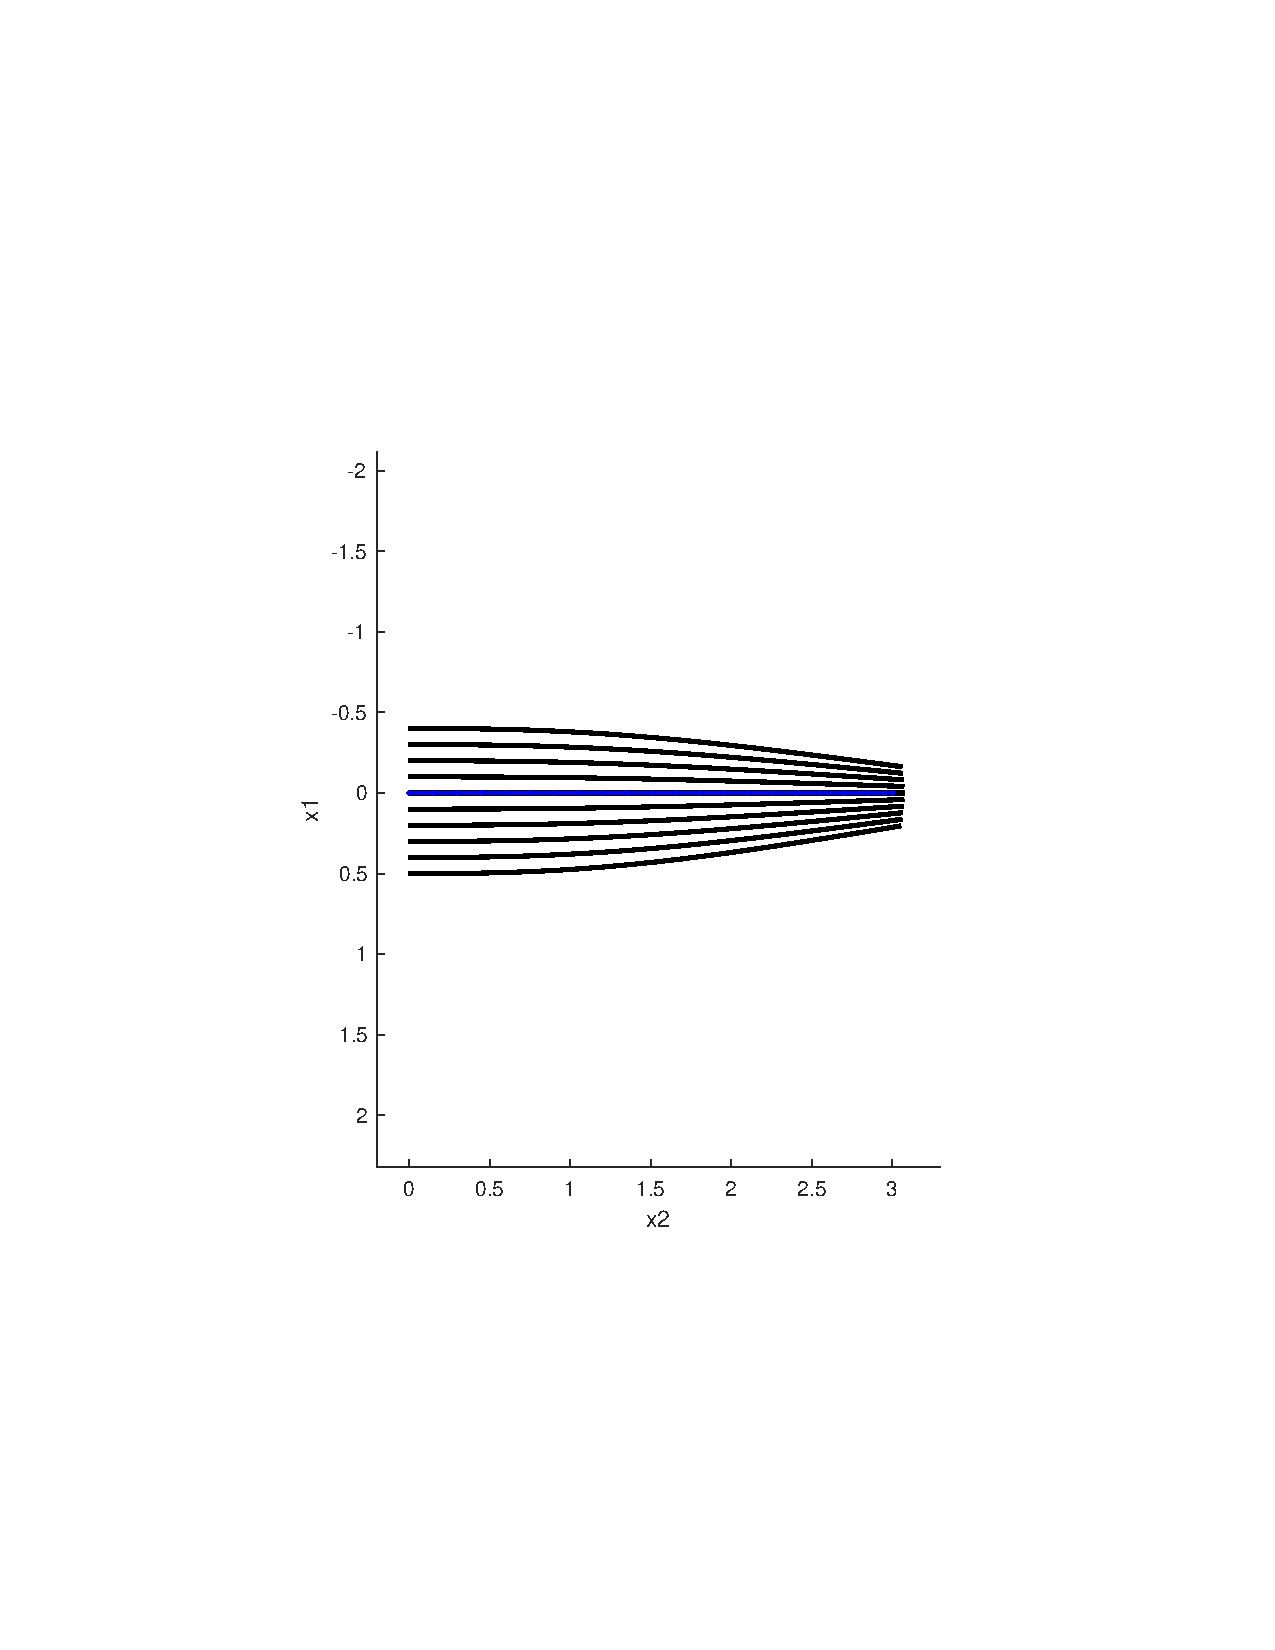
\includegraphics[scale=.5]{figures/Preliminaries/montecarlofunnel}
  \caption{The simulation of N paths starting from a random point in the
    interval \(\sqb{-1,1}\), and controlled with a LQR controller.}
\end{figure}

In this thesis a \textit{Funnel} will refer to the \textit{outer approximation of
forwards reachable sets} parameterized by a \textit{Lyapunov function}.
